\documentclass[12pt]{article}
	
%______________________PREAMBULO_________________________

%----------------------Paquetes--------------------------
\usepackage{amsmath,amssymb,amsfonts,latexsym,cancel} % Paquetes de símbolos adicionales.
\usepackage[spanish,es-tabla]{babel} % Idioma español
\usepackage[utf8]{inputenc} % Paquete que nos permite usar los acentos y otros símbolos, directamente del teclado.
\usepackage[T1]{fontenc} % Cambia el tipo de letra
\usepackage{helvet} % Tipo de letra Arial
\usepackage{graphicx} % Paquete para el manejo de gráficos y figuras en el documento.
\usepackage{geometry} % Permite el manejo de los margenes
\usepackage{fancyhdr} % Permite colocar y manejar el encabezado
\usepackage[breaklinks,colorlinks=true,linkcolor=black,citecolor=blue, urlcolor=blue]{hyperref} % Crea hipervinculo entre secciones y el indice
\usepackage{pstricks}
\usepackage{multicol} % Ayuda a dividir el texto en distintas columnas
\usepackage{float}
\usepackage{bm}
%\usepackage{mathpazo} %fuente palatino
%\usepackage{xcolor}
%\usepackage[shortlabels]{enumitem}
%-------------Paquetes para el formato de las citas-------
%\usepackage[hyphens]{url}
%\usepackage{cite}
%\usepackage{wrapfig}

%-----------------------------ayuda de paquetes--------------------

\spanishdecimal{.} % permite la colocacion de un punto en lugar de una coma en ecuaciones
\renewcommand*\familydefault{\sfdefault} % Ayuda a colocar letra tipo Arial

%------------------------Margenes----------------------------
\newgeometry{bottom = 2.5 cm, top = 2.5 cm, left = 2 cm, right = 2 cm} % Modifica el margen {Abajo, Arriba, Izquierda, Derecha

%----------------------------Interlineado----------------------------------

%\doublespacing
%\onehalfspace
%\singlespace
%\spacing{1.5} % Permite personalisar a gusto
%\setlength{\parskip}{2cm} % Es el espacio entre parrafos

%-----------------------------Sangria---------------------------------------

\setlength{\parindent}{0 cm} % Manipula la sangria

%---------------------Portada------------------

%\title{
%\begin{figure}[h!]
		
%	\centering
%	
\includegraphics[width=\linewidth]{Nom_UAdeC_FCFM.png}  			
			
%\end{figure}
%\huge \textbf{LABORATORIO DE FISICA 3}\\\LARGE TITULO PRACTICA\\}
%\author{ \Large \textbf{Profesor:}\\
%\Large \textbf{Alumno:} Oscar Joel Castro Contreras}
%\date{\today}

%--------------Encabezado y pie de pagina--------------------

\pagestyle{fancy}%Coloca el encabezado en el documento
\lhead[]{Métodos numéricos}%Encabezado izquierda
\rhead[]{Oscar Joel Castro Contreras}%Encabesado derecha
%\chead[]{}%Encabesado central
\renewcommand{\headrulewidth}{0.08 pt}%Coloca linea al pie de pagina

%\lfoot[]{PI}%Pie de pagina izquerdo
%\rfoot[]{PD}%Pie de pagina derecho
\cfoot[]{\thepage}%Pie de pagina central
\renewcommand{\footrulewidth}{0.08 pt}%Coloca linea al pie de pagina

%-----------------------------------------------------------------------------

	\begin{document}
		
		\begin{titlepage}
		
			\centering
			{\bfseries
			\begin{figure}[h!]
				\centering
				
\includegraphics[width=\linewidth]{Nom_UAdeC_FCFM.png} 				
			\end{figure}
			\par}
			\vspace{1cm}
			{\LARGE Métodos numéricos \par}
			\vfill
			{\scshape\Huge \textbf{Conversor de bases} \par}
			\vfill
			{\LARGE \textbf{Profesora:} Maria Guadalupe Godina Cubillo \par}
			\vfill
			{\LARGE \textbf{Alumno:} Oscar Joel Castro Contreras \par}
			\vfill
			{\Large \today \par}
			\thispagestyle{empty}
			%\thispagestyle{fancy}
			
		\end{titlepage}
	
		\newpage
		
		\begin{abstract}
			\noindent En este reporte explico lo que es un sistema numérico, los tipos de sistemas numéricos, como se 
			convierte un número decimal a binario y viceversa y muestro las partes importantes de mi programa 
			en Python hace la conversión de un número de base 10 a uno de base 2 y viceversa.
		\end{abstract}

		\textbf{Palabras clave:} decimal, binario, convertir.

		\begin{center}
			\section*{Introducción}\label{sec:Introducción}
		\end{center}
			El sistema numérico con el que estamos más familiarizados tiene una base 10, el cual, sin duda 
			alguna, resulta de la contabilidad de los diez dedos de las manos. El origen de este sistema data del 
			año 500 d.C., en India, pero con el paso del tiempo esta notación se dispersó a través de Europa 
			como el método predominante de cálculo. Este sistema posee diez símbolos: 0, 1, 2, 3, 4, 5, 6, 7, 8, 9; 
			sin embargo, las computadoras no utilizan esta base numérica para sus cálculos; sino un sistema 
			basado sobre una base dos, el cual tiene solamente dos dígitos: 0, 1. Este sistema numérico de base 
			dos es denominado sistema binario. Pero no fue sino hasta 1945, cuando John Von Neumann 
			estableció el concepto de programa almacenado para las computadoras digitales, que el sistema 
			binario se convirtió en el lenguaje común de todas las computadoras de esa generación y de las 
			futuras.
			El sistema binario es utilizado en las computadoras por las siguientes razones:
			\begin{itemize}
				\item Simplifica los circuitos aritméticos de las computadoras
				\item Proporciona una manera sencilla de almacenar información e instrucciones.
				\item Proporciona confiabilidad.
			\end{itemize}
			Pero cuando se trabaja con computadoras, también se utilizan otros dos sistemas numéricos: 
			hexadecimal y octal, utilizados principalmente como un método para la representación 
			de números binarios:
			\begin{itemize}
				\item \textbf{Sistema numérico decimal:}
					 Está basado en una base de 10 elementos y está compuesto por los dígitos
					 0, 1, 2, 3, 4, 5, 6, 7, 8, 9. La posición de cada cifra, de derecha a izquierda, indica las
					 unidades, decenas, centenas,... Por esta razón, a este sistema también se le llama
					 sistema posicional.
				\item \textbf{Sistema numérico binario:}
					 Esta basado en una base de 2 elementos, el cual se representa por los números 0 y 1.
					 Los números binarios son el sistema común interno de la computación digital debido a la 
					 relativa simplicidad de registrar, almacenar y reconocer variables de sólo dos valores.
				\item \textbf{Sistema numérico octal:}
					 Se basa en una base de 8 elementos y utiliza los dígitos 0, 1, 2, 3, 4, 5, 6, 7. Este sistema 
					 tiene características especiales que lo hacen muy útil en muchas situaciones que involucran 
					 números binarios. Puesto que tres dígitos binarios se agrupan y representan un dígito octal.
					 En la tabla 1 se muestra cómo son utilizados los dígitos octales para la representación de 
					 agrupaciones de tres dígitos.
					\begin{table}[h!]
						\centering
						\begin{tabular}{|c|c|}
							\hline
							Octal & binario \\\hline
							1 & 000 \\\hline
							1 & 001 \\\hline								
							2 & 010 \\\hline
							3 & 011 \\\hline
							4 & 100 \\\hline
							5 & 101 \\\hline
							6 & 110 \\\hline
							7 & 111 \\\hline
						\end{tabular}
						\caption{Equivalencia de un digito octal en binario}
						\label{tab:1}
					\end{table}
				\item \textbf{Sistema numérico hexadecimal:}
					 El sistema numérico hexadecimal se basa en una raíz 16, por lo que emplea 16 dígitos: 0, 1, 2, 
					 3, 4, 5, 6, 7, 8, 9, A, B, C, D, E, F; en éste, los dígitos del 0 al 9 se usan en sentido 
					 normal y los otros seis dígitos, representados por las letras A, B, C, D, E, F, se utilizan 
					 con equivalencia (A = 10, B = 11, C = 12, D = 13, E = 14, F = 15). Como en el sistema octal 
					 existe una equivalencia entre un digito hexadecimal y binario, en la tabla 2 se muestra la 
					 equivalencia de un digito hexadecimal respecto al sistema binario.
					 \begin{table}[h!]
						\centering
						\begin{tabular}{|c|c|}
							\hline
							Octal & binario \\\hline
							1 & 0000 \\\hline
							1 & 0001 \\\hline
							2 & 0010 \\\hline
							3 & 0011 \\\hline
							4 & 0100 \\\hline
							5 & 0101 \\\hline
							6 & 0110 \\\hline
							7 & 0111 \\\hline
							8 & 1000 \\\hline
							9 & 1001 \\\hline
							A & 1010 \\\hline
							B & 1011 \\\hline
							C & 1100 \\\hline
							D & 1011 \\\hline
							E & 1110 \\\hline
							F & 1111 \\\hline
						\end{tabular}
						\caption{Equivalencia de un digito hexadecimal en binario}
						\label{tab:2}
					\end{table}
			\end{itemize}

		\begin{center}
			\section*{Metodología}\label{sec:Metodología}
		\end{center}
			\begin{itemize}
				\item \textbf{Convercion de Decimal base 10 a Binario base 2:}\\
					 Para convertir números decimales a binarios, lo primero es separar el parte entero y la parte 
					 fraccionaria del número decimal ya que la parte entera se convierte a binario de una forma distinta 
					 que la parte fraccionaria.\\
					 Para la parte entera el procedimiento consiste en dividir entre dos la parte entera y guardar el 
					 residuo, después debes obtener la parte entera del cociente de la división anterior, luego volver a 
					 dividir entre 2 y guardar su residuo y así sucesivamente hasta que el entero del cociente de es cero. 
					 El residuo siempre saldrá como 0 o 1, estos 0 y 1 obtenidos se van acomodando de izquierda a derecha 
					 y así se va formando el número binario que representa a la parte entera del número decimal.\\
					 Para la parte fraccionaria el procedimiento consiste en multiplicar por dos, después le debes guardar 
					 la parte entera del resultado y restársela al resultado de la multiplicación, luego de nuevo debes 
					 multiplicar por dos el resultado de la resta, guardar su parte entera y restársela al resultado de la 
					 multiplicación, así sucesivamente hasta que el resultado de la resta es igual a cero, hay ocasiones 
					 en las que nunca se hace cero por lo que se debe elegir una cierta cantidad de veces para las que se 
					 hará este procedimiento. Lo número esteros guardados siempre será 0 y 1 y se acomodan después 
					 de un punto de derecha a izquierda y así se va formando el número binario que representa a la parte 
					 fraccionaria del número decimal.\\
					 Al final solo debes sumar los números binario obtenidos de cada parte.
				\item \textbf{Convercion de Decimal base 2 a Binario base 10:}
					 Para convertir un número binario a decimal, es igual que antes, primero debes separa la parte entera 
					 y la parte fraccionaria del número binario.\\
					 Para la parte entera el procedimiento consiste en tomar cada digito de la parte entera del número 
					 y multiplicarla por 2 a la potencia del número de la posición del digito, empezando a contar de 0 y 
					 de derecha a izquierda, después sumamos todos los resultados de las operaciones realizadas a cada 
					 digito del número y obtenemos el número decimal.\\
					 Para la parte fraccionaria el procedimiento es casi el mismo que para la parte entera solo que la 
					 potencia es negativa, se empieza a contar desde 1 y de izquierda a derecha, y obtenemos la parte 
					 fraccionaria.\\
					 Al final solo debes sumar los números decimales obtenidos de cada parte.
			\end{itemize}

			\newpage

		\begin{center}
			\section*{Resultado}\label{sec:Resultado}
		\end{center}
			Esta parte de mi programa recibe la parte entera del número decimal y la convierte a binario:
			\begin{center}
				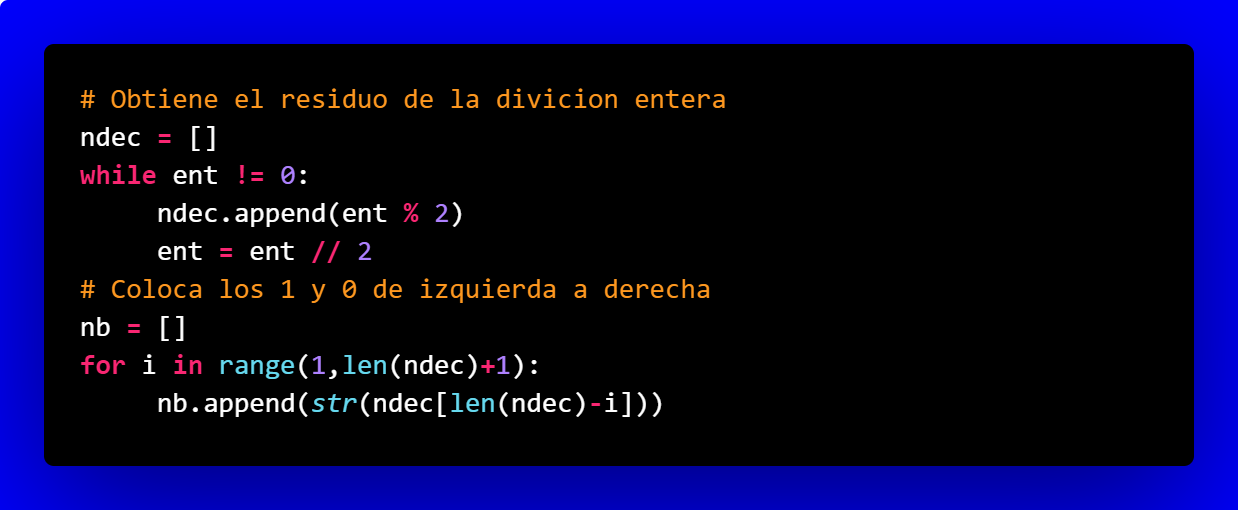
\includegraphics[width=\linewidth]{Base 10 a Base 2.png} 				
			\end{center}
			Esta parte de mi programa recibe la parte fraccionaria del número decimal y la convierte a binario:
			\begin{center}
				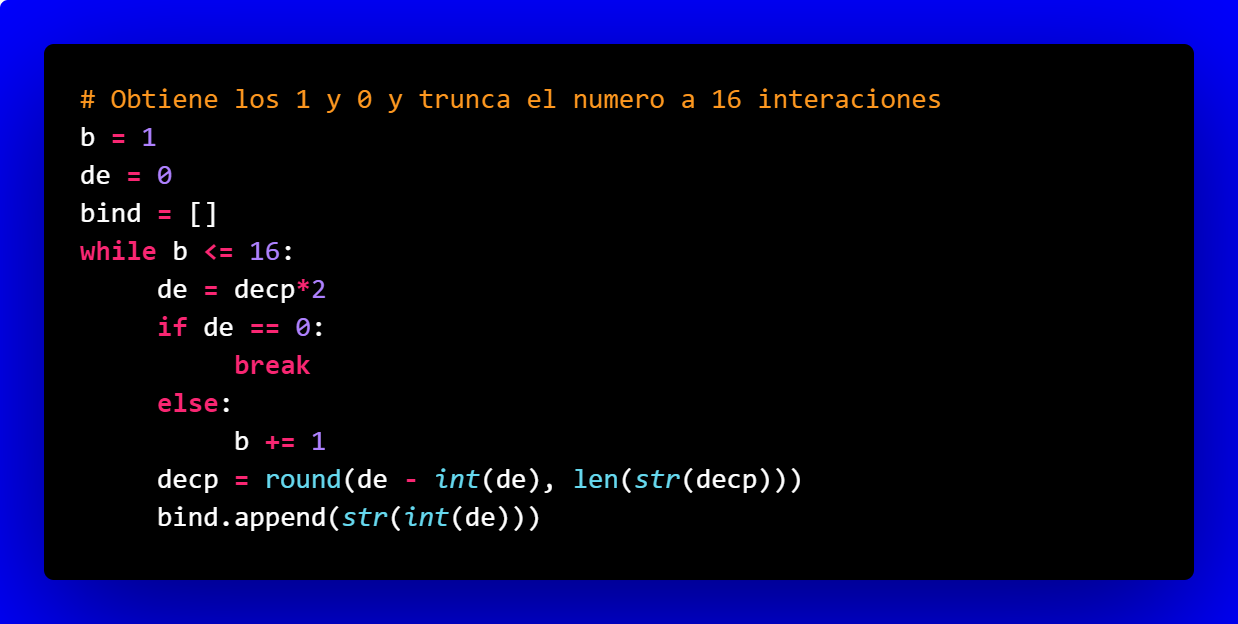
\includegraphics[width=\linewidth]{Basef 10 a Basef 2.png} 				
			\end{center}
			\newpage
			Esta parte de mi programa toma la parte entera del número binario y la convierte a decimal:
			\begin{center}
				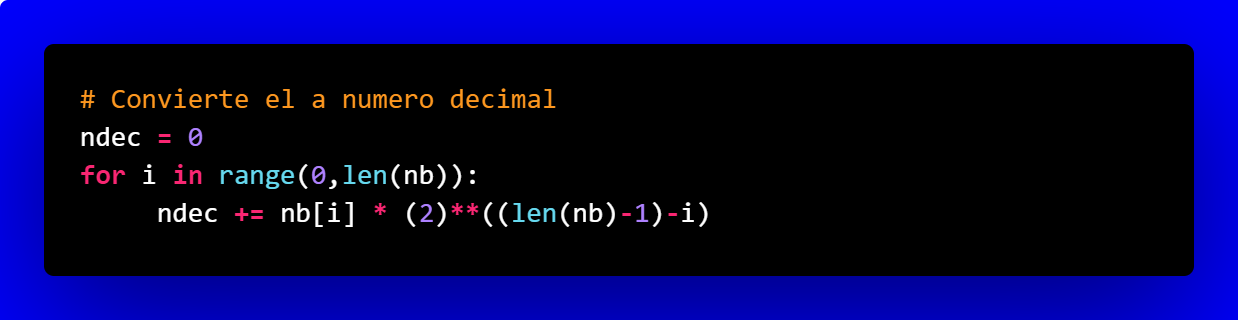
\includegraphics[width=\linewidth]{Base 2 a Base 10.png} 				
			\end{center}
			Esta parte de mi programa toma la parte fraccionaria del número binario y la convierte a decimal:
			\begin{center}
				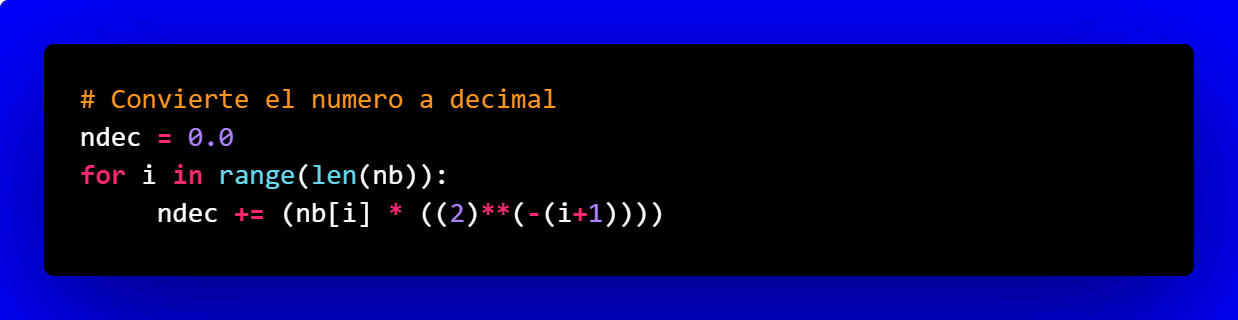
\includegraphics[width=\linewidth]{Basef 2 a Basef 10.png} 				
			\end{center}

		\begin{center}
			\section*{Conclusión}\label{sec:Conclusión}
		\end{center}
			En conclusión, se puede ver que cuando la computadora realiza todo este proceso recibir un número 
			decimal, lo convierte a binario, hace las tareas que se le indicaron hacer con un número binario y 
			volver a convertir a decimal el resultado de la tarea que se le indico, se pierden mucha información, 
			por lo que esta es una de las razones por la que se debe tener cuidado con los errores que tiene la 
			computadora a la hora de realizar cualquier tarea.\\

		\centering
		\begin{thebibliography}{10}
			\bibitem{bib:item1} Olvera, M. A. C., Rodríguez, A. C., González, J. A. R., y Gutiérrez, A. C. V. (2014). Fundamentos de
							Computación para Ingenieros. Grupo Editorial Patria.
			
		\end{thebibliography}

	\end{document}